%\documentclass[sigconf,screen]{acmart} 
\documentclass[sigconf,review, anonymous]{acmart}
% \documentclass[sigconf,review]{acmart}

%\usepackage[latin1]{inputenc}
\usepackage{graphicx}
%\usepackage{algorithm}
\usepackage[linesnumbered,ruled,vlined]{algorithm2e}
\usepackage{algorithmic}
\usepackage{multirow}
\usepackage{longtable}
\usepackage{rotating}
\usepackage{enumerate}
%\usepackage{slashbox}
%\usepackage{amsthm}
\usepackage{amsmath}
\usepackage{xcolor}
\usepackage{epstopdf}
\usepackage{subfigure}
\usepackage{listings}
\usepackage{xcolor}
\usepackage{url}
\usepackage{caption}
\usepackage{hyperref}
\usepackage{slashbox,multirow}
\usepackage{flushend}
%\reference alignment
\definecolor{keywordcolor}{rgb}{0,0,1.0}
\definecolor{lightgreen}{rgb}{0,0.8,0}
\definecolor{webgreen}{rgb}{0,0.5,0}

\newcommand{\tabincell}[2]{\begin{tabular}{@{}#1@{}}#2\end{tabular}}  

\newcommand{\hytt}[1]{\texttt{\hyphenchar\font=\defaulthyphenchar #1}}
\newtheorem{definition}{Definition}
\newtheorem{pattern}{Anti-pattern}

\lstset{
  language=Java,
  alsolanguage= XML,
  tabsize=4, %
  frame=, %把代码用带有阴影的框圈起来
  %rulesepcolor=\color{red!20!green!20!blue!20},%代码块边框为淡青色
  keywordstyle=\color{red!20!green!20!blue!20}, %代码关键字的颜色为蓝色,粗体
  showstringspaces=false,%不显示代码字符串中间的空格标记
  stringstyle=\ttfamily, % 代码字符串的特殊格式
  keepspaces=true, %
  breakindent=22pt, %
  %frame=single,
  numbers=left,%左侧显示行号 往左靠,还可以为right,或none,即不加行号
  stepnumber=1,%若设置为2,则显示行号为1,3,5,即stepnumber为公差,默认stepnumber=1
  %numberstyle=\tiny, %行号字体用小号
  numberstyle={\color[RGB]{0,204,0}\tiny} ,%设置行号的大小,大小有tiny,scriptsize,footnotesize,small,normalsize,large等
  numbersep=8pt,  %设置行号与代码的距离,默认是5pt
  commentstyle={\color{green}\tiny},%浅灰色的注释
  basicstyle=\footnotesize, % 这句设置代码的大小
  showspaces=false, %
  flexiblecolumns=true, %
  breaklines=true, %对过长的代码自动换行
  breakautoindent=true,%
  breakindent=4em, %
  %aboveskip=1em, %代码块边框
  tabsize=2,
  showstringspaces=false, %不显示字符串中的空格
  fontadjust,
  framextopmargin=2pt,framexbottommargin=2pt,abovecaptionskip=-3pt,belowcaptionskip=3pt,
  xleftmargin=1em,xrightmargin=1em, % 设定listing左右的空白
}

\lstset{language=[AspectJ]Java,
basicstyle=\footnotesize,
keywordstyle=\color{keywordcolor}, %\underbar,
identifierstyle=,
commentstyle=\color{lightgreen} \textit,
stringstyle=\ttfamily,
showstringspaces=false,
captionpos=b
}


\copyrightyear{2020} 
\acmYear{2020} 
\setcopyright{acmcopyright}
\acmConference[ICSE'20]{Proceedings of the 42nd International Conference on Software Engineering}{May 23--29, 2020}{Seoul, South Korea}
\acmPrice{15.00}
%\acmDOI{10.1145/3338906.3338950}
%\acmISBN{978-1-4503-5572-8/19/08}


\begin{document}
\title{TNBDroid: Testing HTTP(S) Network-Related Behaviour of Android Applications}
%\titlenote{Produces the permission block, and copyright information}
%\subtitle{Extended Abstract}
%\subtitlenote{The full version of the author's guide is available as \texttt{acmart.pdf} document}


\author{Wei Song}
%\authornote{Dr.~Trovato insisted his name be first.}
\orcid{0000-0002-4324-3382}
\affiliation{%
  \institution{School of Computer Sci. \& Eng.\\Nanjing University of Sci. \& Tech.}
  %\streetaddress{Xiaolingwei 200}
  \city{Nanjing}
  %\state{Ohio}
  \country{China}
  \postcode{210094}
}
\email{wsong@njust.edu.cn}

\author{Jing Zhang}
%\authornote{Dr.~Trovato insisted his name be first.}
\affiliation{%
  \institution{School of Computer Sci. \& Eng.\\Nanjing University of Sci.\& Tech.}
  %\streetaddress{Xiaolingwei 200}
  \city{Nanjing}
  %\state{Ohio}
  \country{China}
  %\postcode{210094}
}
\email{zjing8017@gmail.com}

\author{Jeff Huang}
%\authornote{This author is the one who did all the really hard work.}
\affiliation{%
  \institution{Parasol Laboratory\\Texas A\&M University}
  %\streetaddress{1 Th{\o}rv{\"a}ld Circle}
  \city{College Station, TX}
  \country{USA}
  }
\email{jeff@cse.tamu.edu}


% The default list of authors is too long for headers.
%\renewcommand{\shortauthors}{}


\begin{abstract}
For most Android apps, while the network plays a critical role in providing the app functionalities, the bugs of network usage account for a large proportion of app crashes. Since many network-related bugs can only be triggered in certain conditions (e.g., when the network speed is slow, the network response takes a long latency), it is difficult for existing general or GUI testing approaches to manifest them. To the best of our knowledge, there are few techniques dedicated to testing the network usage in apps. In this paper, we present an automatic traversal-based testing approach, \textsf{TNBDroid}, to effectively and efficiently explore the HTTP(S) network-related behaviour of apps. We have applied \textsf{TNBDroid} to 35 real-world Android apps, and the experimental results demonstrate that our approach achieves a high coverage (on average 77.37\%) of the HTTP(S) network-related behaviour, and totally finds from the 35 apps 57 bugs that are relevant to the HTTP(S) network usage in 683 minutes.
\end{abstract}

%
% The code below should be generated by the tool at
% http://dl.acm.org/ccs.cfm
% Please copy and paste the code instead of the example below.
%
\begin{CCSXML}
<ccs2012>
<concept>
<concept_id>10011007.10011074.10011099.10011102.10011103</concept_id>
<concept_desc>Software and its engineering~Software testing and debugging</concept_desc>
<concept_significance>500</concept_significance>
</concept>
</ccs2012>
\end{CCSXML}

\ccsdesc[500]{Software and its engineering~Software testing and debugging}

%\ccsdesc[500]{Software and its engineering~Software defect analysis}


\keywords{Android app, network-related behaviour, testing}

\maketitle

\section{Introduction}
Many Android apps (apps for short) are built to replace the corresponding Web applications running on the desktop in the traditional client(browser)-server model. Therefore, these apps call for network to connect to the server to download and upload resources, and to update and share data to others.  Since the network is diverse (e.g., 2G/3G/4G, WiFi,  Bluetooth) and could be unstable, apps tend to crash due to network problems and exceptions~\cite{LBZKLLTSCZ14,XiongCZXQ18,HuangZJLL19}. Thus, app developers and testers should pay attention to the network invocations and the relevant behaviour of apps.

Although many techniques and tools have been proposed for testing apps, they are mostly general testing approaches, mainly focusing on testing the GUI of apps~\cite{ChoudharyGO15,WangLYCZDX18}. When they (e.g., \textsf{Monkey}~\cite{monkey}) are used to test apps, much network-related behaviour cannot be explored effectively or efficiently. On the other hand, there are few approaches dedicated to the testing of network-related behaviour of apps. For example, Huang et al. employ the middleman technique to simulate different response data for detecting the network security threats to apps~\cite{HuangZJLL19}. However, the middleman technique is forbidden by many apps.  

In practice, app developers test network-related behaviour of apps in manual ways or with the help of different hardware and software simulators~\cite{LBZKLLTSCZ14,XiongCZXQ18,HuangZJLL19}. Specifically, they usually set different network environments to test the network-related behaviour of apps, and also validate the app when the network switches to another kind. Besides, they may also change the physical properties of the network (e.g., limit the speed of the network, increase the network response latency) to check whether their apps crash in such scenarios. Although this practice can manifest some bugs that are relevant to the network usage, it is resource-intensive and time-consuming. More importantly, this approach cannot test the network-related behaviour systematically because it is difficult to simulate all network environments, and thus some potential network-related bugs may not be found. 

A study reports that in the app crash with the network call, about 88\% of the network calls are successful, but returned unexpected data (dirty data); and, 10\% of successful network calls that return no data\footnote{https://www.apteligent.com/research/network-crashes (accessed Aug, 2018)}. Inspired by these, we propose in this paper a traversal-based testing approach, and an open-source tool \textsf{TNBDroid} (the URL is omitted for double-blind review), to systematically and automatically test the HTTP(S) network-related behaviour of apps. Our approach is based on the techniques of fuzzing, a technical to manifest program bugs by iteratively providing irregular data to the program~\cite{CorinaMSSHKV17,HuangZJLL19}. Our main idea is to use a software-defined way to instrument an app to define different possible outcomes (e.g., response data) of the HTTP(S) network request, and see how apps respond to the different outcomes (whether apps work well in the presence of different outcomes). The rationale behind lies in that many app crashes are not caused by the network itself or its properties (e.g., speed), but due to the fact that the app code does not handle the network exceptions or the response data in a proper way. As a consequence, we do not need to simulate different kinds of networks or their specific properties; instead we can directly simulate the possible responses of the HTTP(S) network request. 

To implement our approach, we first conduct a static analysis of the app to locate the positions of all HTTP(S) network requests (i.e., network API invocations) based on \textsf{Soot}~\cite{sootpaper}\footnote{https://github.com/Sable/soot}. Meanwhile, we also determine the impact scope (in terms of a set of statements, called slice) of each network request. Based on the position of each HTTP(S) network API invocation, we then instrument the original app to add some code at the position to acquire the real response data based on which we can do fuzzing (i.e., define other possible response data) accordingly. Based on \textsf{Robotium}\footnote{https://github.com/RobotiumTech/robotium},  we pre-explore the app to identify the activities that do not trigger network request directly. In the real traversal-based testing, these activities can be skipped to improve the exploration efficiency. Note that all simulated response data is supposed to be handled by the corresponding HTTP(S) network-related behaviour of the app. If the app does not handle the response data properly, a bug can be found.      

The contributions of this work are summarized as follows:
\begin{enumerate}
\item We develop a traversal-based testing approach and an open-source tool \textsf{TNBDroid} to systematically and automatically test the HTTP(S) network-related behaviour of apps. Based on a static scan and the following instrumentation, our approach traverses the app to first record the real network response data and then simulate and mutate the other possible response data accordingly with a set of fuzzing rules, which can test the network-related behaviour in an efficient and low-cost way.
\item We apply \textsf{TNBDroid} to 25 apps from F-droid and 10 commercial apps from Google Play, the results of which demonstrate both the effectiveness and efficiency of our approach: it achieves a high code coverage (on average 81.74\% for apps from F-droid, 66.43\% for apps from Google Play) of the HTTP(S) network-related behaviour, and totally finds 57 bugs relevant to the network usage in the 35 apps.
\end{enumerate}    


The remainder of the paper is organized as follows. Section~\ref{relatedwork} positions our study in the related work.
Section~\ref{approach} presents our approach to testing network-related behaviour of apps.
Section~\ref{evaluation} reports on the experimental results on real-world apps. Section~\ref{limitation} discusses the limitations of our current work, and Section~\ref{conclusion} concludes the paper.

\section{Related Work}\label{relatedwork}
Our work is related to both network behaviour analysis and automated testing of Android apps. In this section, we briefly review the existing work on these two aspects.

\subsection{Network Behaviour Analysis}
%Let us first review the work on network behaviour analysis and testing for mobile (Android) apps. 

\textbf{Network behaviour analysis}. Nayam et al.~\cite{NayamLCS16} present a framework for identifying undesirable network behaviour of mobile apps. The proposed framework runs an app to obtain packet-level traces of the app's network behaviour, and then generates a set of attributes to group the app behaviour into three categories, including suspicious, potentially suspicious, and innocuous. Mostafa et al.~\cite{MostafaRW17} propose a method for statically summarizing network behaviour from the bytecode of Android apps, which can be used to determine the location of network-related code in the apps and to facilitate the maintenance of such code. Based on the string taint analysis, the method generates a summary of the network request by statically estimating the possible values of the network API parameters. The method is implemented as a static analysis tool \textsf{NetDroid}.

%Some work focuses on the collection of network traffic, which is also relevant to the network analysis in a broad sense. For example, Dai et al.~\cite{DaiTWNS13} propose and implement a tool, called \textsf{NetworkProfiler}, to automatically generate network traffic profiles for Android apps. Specifically, it uses a UI fuzzing technique to automate the execution of the app, and meanwhile collects network traffic generated by the app.  Su et al.~\cite{SuZLW15} develop an automated Android network traffic generation system, called \textsf{AndroGenerator} to acquire various types of network traffic generated by Android apps. They also extract some network features from the captured network traffic, which can be used for other research, e.g., for identifying Android apps.

\textbf{Network behaviour testing}. To test the network behaviour of mobile apps, the main method is to simulate various network environments through hardware or software, and then run the app in the simulated network environment to verify whether errors will occur. For example, \textsf{Caiipa}~\cite{LBZKLLTSCZ14} is based on the cloud service technology for testing mobile app over an expandable mobile context space. It simulates various contexts including various network environments at the hardware level. 
Some existing middle agent software, such as \textsf{Fiddler}\footnote{https://www.telerik.com/fiddler} and \textsf{Charles}\footnote{https://www.charlesproxy.com}, can capture network data and simulate different network issues, such as long network latency and network low bandwidth. App developers often utilize these software to approximately simulate the bad network environment and use the captured network data to determine the success and failure of the network request. 


There are also some work which simulates network failures by injecting network-related exceptions into the app. For example, Yang et al.~\cite{Yang2013Testing} study the impact of weak response on the app, and detect whether the app can have an ANR (Application Not Responding) error by inserting a long delay into the typical time-consuming operation (including network access) in the app. Similarly, \textsf{JazzDroid} is an automated Android gray box testing tool that dynamically injects various environmental interference into the application to detect issues~\cite{XiongCZXQ18}. It contains a network issues injector that interferes with the app's HTTP requests and manipulates their responses to simulate network latency and connectivity. 

In contrast to these researches, we do not simulate the network environments or the network issues such as network latency and connectivity. Instead, we directly simulate the response data that could be generated in those scenarios. Therefore, our approach is more easy to implement. 
Similar to us, Huang et al.~\cite{HuangZJLL19} propose a network packet-based fuzzing method to test the network-related behaviour of Android apps. Based on \textsf{Monkey} and the middleman technique, this method first obtains the interaction data sent by servers to apps, and then adopts different mutation strategies to mutate the original data, and finally returns the mutated response data to apps. However, the middleman technique can only intercept the network data from the port in the WiFi environment, and thus it is difficult to know which app the data belongs to. 
The goal is to discover potential security threats of the apps. By contrast, our goal is to test network-related behaviour as comprehensively and efficiently as possible, not just to discover potential threats.


\subsection{App Testing}

Most existing app testing approaches aim at  
detecting general (UI) bugs that can be triggered from the app GUI~\cite{ChoudharyGO15,WangLYCZDX18}. Their goal is to explore the app behaviour as comprehensively as possible. Generally speaking, there are three exploration strategies used in app testing\cite{ChoudharyGO15}: \textit{random testing}~\cite{monkey,MachiryTN13,SongQH17}, \textit{model-based testing}~\cite{GUIRipping,grey-box,SuMCWYYPLS17,GuSMC0YZLS19}, and \textit{event sequence-based testing}~\cite{AnandNHY12,EvoDroid,MaoHJ16}. 

\textbf{Random testing}. \textsf{Monkey}~\cite{monkey} provided together with the Android SDK is the most frequently-used testing approach for Android apps~\cite{ChoudharyGO15}. However, \textsf{Monkey} generates many redundant events in the testing. To this end, \textsf{Dynodroid}~\cite{MachiryTN13} is proposed to reduce the generation of redundant events. It triggers the next event based on the app reaction of the preceding triggered event. Since it is difficult to trigger certain events from the GUI, \textsf{EHBDroid}~\cite{SongQH17} is proposed to directly trigger the event callbacks (event handlers) based on the app instrumentation. Although \textsf{EHBDroid} bypasses the GUI and thus is more efficient, its random testing may generate false alarms because some bugs it detects do not occur in real executions. Besides these studies, the early Android app testing approaches mostly fall into the category of random testing~\cite{HuN11,AmalfitanoFT11,GUIRipping,flowdroid}. 

\textbf{Model-based testing}. Since redundant events are inevitably generated in random testing, a great deal of work propose to use model-based testing~\cite{GUIRipping,grey-box,ChoiNS13,a3e,Guided,BaekB16,SuMCWYYPLS17,GuSMC0YZLS19}. These approaches rely on a model (e.g., a state machine) of the app GUI to generate test cases. The models are either obtained manually or can be generated through static and dynamic program analysis techniques. For example, \textsf{GUIRipper}~\cite{GUIRipping} dynamically builds such a model based on which a depth-first exploration strategy is employed to test the app. \textsf{GUIRipper} is a black-box approach limited to UI event generation. \textsf{ORBIT}~\cite{grey-box} first derives a model based on the app source code, and then utilizes the model to generate event for testing. \textsf{Stoat}~\cite{SuMCWYYPLS17} is a guided approach to performing stochastic model-based testing on apps. Recently, a new model-based testing tool, called \textsf{Ape}, is presented~\cite{GuSMC0YZLS19}. Instead of using a static model, \textsf{Ape} dynamically optimizes the model based on the generated information during testing.  
The effectiveness of these approaches significantly depends on the model. However, it is rather difficult to derive a accurate and complete model of the app. 


\textbf{Event sequence-based testing}. Since many well-hidden bugs can only be manifested through specific event sequences. The last category approaches focus on generating such event sequences for app testing~\cite{AnandNHY12,JensenPM13,EvoDroid,MaoHJ16}. For instance,  \textsf{ACTEve}~\cite{AnandNHY12} employs the technique of symbolic execution to generate effective event sequences. 
\textsf{EvoDroid}~\cite{EvoDroid} leverages the evolutionary algorithm to generate specific event sequences. \textsf{Sapienz}~\cite{MaoHJ16} uses a search-based algorithm to yield a set of shortest event sequences which can maximize the code coverage.

Recently, some work focuses on testing certain properties of apps, e.g., energy testing~\cite{BehrouzSBM16,BanerjeeCBR18,JabbarvandLM19}, service testing~\cite{ZhangLLC17,ma2018}. However, little work concentrates on network-related behaviour testing. 


\section{TNBDroid}\label{approach}

Figure~\ref{fig_framework} shows the workflow of our approach \textsf{TNBDroid}. The input of \textsf{TNBDroid} is an Android app, and the output is a crash (bug) report and a code coverage report for the HTTP(S) network-related behaviour. \textsf{TNBDroid} involves the following four major stages (modules), where the first two steps are based on \textsf{Soot}\footnote{https://github.com/Sable/soot} if the source code is unavailable, and the last two are based on \textsf{Robotium}\footnote{https://github.com/RobotiumTech/robotium}. 
\begin{enumerate}
\item \textbf{Static analysis}. It locates in the app the positions of all HTTP(S) network API invocations. Moreover, for each API invocation, it utilizes a program slicing tool to determine the slice (a set of statements) that could be impacted by the network API invocation.    
\item \textbf{Instrumentation}. This stage instruments the original app to obtain two new apps: the pre-explored app and the tested app. The exploring app is obtained as follows. For each HTTP(S) network API invocation, it instruments a logging statement to indicate whether this invocation is executed at runtime. The testing app is obtained in the following way. For each HTTP(S) network API invocation, it instruments some statements that records the response data for the invocation, and simulates and mutates some other possible response data. 
\item \textbf{Pre-exploration}. In this stage, the pre-explored app is employed to identify the activities that do not trigger HTTP(S) network API invocations. Specifically, it dynamically explores the app using a breadth-first traversal (details are in the following) and records the activities that are visited. It also labels each visited activity to indicate whether network API invocations can be triggered directly from the activity, which is helpful for reducing the  space of the testing. 
\item \textbf{Testing}. Based on the output of the auto-exploration stage, this stage explores the tested app by a breadth-first traversal to trigger all HTTP(S) network API invocations and the following behaviour. It also substitutes the instrumented response data for the real response data to sufficiently test the relevant behaviour of the API invocations. Its output is a crash report and a code coverage report.   
\end{enumerate}

\begin{figure}
 \centering
  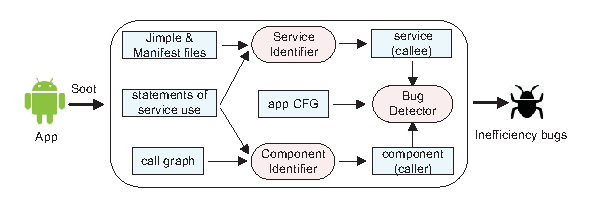
\includegraphics[scale=0.6]{framework.eps}
  \caption{Framework of \textsf{TNBDroid}.}
  \label{fig_framework}
\end{figure}

In the following, we elaborate on these four stages, respectively. 


\subsection{Static Analysis}\label{sub_staticanalysis}
The static analysis is performed on the source code of the app. If only the APK file is available, the static analysis can be applied to the Jimple code. This stage involves the following two steps.

\textbf{Network API localization}. Android SDK provides a variety of network APIs. App developers can choose appropriate network APIs to make app access to the network. Additionally, certain apps may also use third-party frameworks to connect to the network. To systematically test all the network-related behaviour of an app, we first need to determine which network APIs are used in the app, and where they are used. The network APIs considered in this paper are summarized in Table~\ref{tab:APIs}, including the native APIs of Android SDK and the APIs of the three most popular third-party network libraries, where concrete methods of the APIs are not listed. Since the return data type of \texttt{java.net.Socket} is not known, we do not consider the APIs of socket communications. In the following, when we mention network requests and network API invocations, they all refer to HTTP(S) requests. When the source code of the app is not available, we use \textsf{Soot} to convert the app's bytecode into the Jimple code. The Jimple code is more readable than the bytecode and is more suitable for program analysis. We traverse the Jimple code to locate the positions (called target points) where the network APIs are used in the app.

\begin{table} 
\centering
\small
\caption{Android Network APIs} %标题
\begin{tabular}{|l|l|}
\hline
{\bf Category} & {\bf Class}   \\
\hline
\hline
\multirow{4}{*}{Android SDK} & {\texttt{java.lang.URL}}\\
\cline{2-2}
&  \tabincell{l}{\texttt{java.net.URLConnection}\\\texttt{java.net.HttpURLConnection}\\\texttt{javax.net.ssl.HttpsURLConnection}} \\
\cline{2-2}
&  \texttt{org.apache.http.client.HttpClient} \\
\cline{2-2}
&  \texttt{java.net.Socket} (not considered) \\
\cline{2-2}
\hline
\multirow{3}{*}{Android network libraries} & {\texttt{Retrofit}}  \\
\cline{2-2}
&  \texttt{Volley} \\
\cline{2-2}
&  \texttt{OkHttp} \\
\cline{2-2}
\hline
\end{tabular}
\label{tab:APIs}
\end{table}

\textbf{Forward slicing}. The behaviour of an app is very complicated, while the network-related behaviour is only a part of it. Since our goal is to manifest the bugs relevant to the network usage, we only focus on the app code that corresponds to the network-related behaviour. To this end, we use an open source tool, called \textsf{Extractocol}~\cite{KimCNCCHKLH16}\footnote{https://github.com/kaist-ina/Extractocol\_public}, to extract the program slice $s_r$ (a set of statements) with respect to each network request and the corresponding response. \textsf{Extractocol} is based on \textsf{Flowdroid}~\cite{flowdroid}\footnote{https://github.com/secure-software-engineering/FlowDroid}. Since the bugs of network usage are mainly caused by the network response data, we use the forward slicing technique of \textsf{Extractocol} to obtain all statements that could be affected by the network response data. The network-related behaviour is reflected and determined by the statements of network requests and the statements in the corresponding slices.
%which are recorded as Response slices.


\subsection{Instrumentation}\label{sub_instrumentation}
This stage is to prepare two instrumented apps for the last two stages, respectively. Similar to the stage of static analysis, the instrumentation can be applied to the source code, or the Jimple code with the help of \textsf{Soot}. 

\textbf{Logging statement insertion}. As aforesaid, by running the pre-explored app at the third stage, we can determine which activities can directly trigger network requests and which cannot. To obtain the pre-explored app, we need to instrument the original app by adding a log statement at each of the target points identified in the first stage.  By running the pre-explored app, once the app initiates a network request, the corresponding log statement will be printed. The printed log is captured in real-time with the help of the Android debugging tool \textsf{ADB}\footnote{https://developer.android.com/studio/command-line/adb}. At the third stage (pre-exploration) of our approach, if during the lifecycle of an activity, there is a log captured by \textsf{ADB}, it indicates that the activity can directly trigger network request and referred to as the network activity.

%If only the APK file is available, we use the instrumentation technique provided by \textsf{Soot} to achieve the instrumentation.

\textbf{Response data recording and fuzzing}. As aforesaid, by running the tested app at the four stage, we can validate whether the app can properly handle different response data of the network request. To obtain the tested app,  
we instrument the app to implement the function of automatically acquiring network response data and the follow-up fuzzing. Meanwhile, we also instrument an log statement for each statement in the slice $s_r$ (returned in the first stage) of each network request, in order to calculate the code coverage of our approach. More details are as follows.

\textit{Instrumentation point}. Since an app may use multiple network APIs, we need to instrument the data acquisition and fuzzing code in all of the app's network API calls to test the network-related behaviour of the app as comprehensively as possible. For native network APIs (Android SDK), the instrumentation is performed at the corresponding target point (strictly speaking, at the position directly follows the target point). Since the \texttt{Volley}\footnote{https://github.com/google/volley} library encapsulates the Android SDK for the network request, the instrumentation point is determined in the way similar to the  native network APIs. For apps that use the libraries \texttt{Retrofit}\footnote{https://square.github.io/retrofit} and \texttt{OkHttp}\footnote{https://square.github.io/okhttp}, since both libraries provide synchronous and asynchronous APIs for network request, and it is somewhat difficult to obtain the response object for the asynchronous request, the target point identified in the first stage cannot be the correct instrumentation point. We choose to instrument inside the library. Since \texttt{Retrofit} uses \texttt{OkHttp} for the network request, we can only instrument \texttt{OkHttp} accordingly. In \texttt{OkHttp}, no matter whether synchronous or asynchronous network request is used, the  \texttt{getResponseWithInterceptorChain()} method is finally invoked, in which we choose the statement that invokes the \texttt{proceed()} method as the instrumentation point, because it returns the response object for the network request.  

\textit{Response data acquisition}. Our method is mainly for the network request based on the HTTP(S) protocol. The response of HTTP(S) contains not only the response data, but also the status code and response header\footnote{https://en.wikipedia.org/wiki/Hypertext\_Transfer\_Protocol}. We determine whether the network request is successful according to the status code, and judge whether the response data is empty according to whether ``Content-Length'' in the response header is zero. From the ``Content-Type'' field in the response header, we know the type of response data. Based on this information, we can parse the response data correctly and perform the follow-up data fuzzing. For the socket communication, since only the data stream is returned, it is not easy to perform fuzzing. Therefore, we do not consider APIs of socket communication. 

\textit{Response data fuzzing}. Since most crashes relevant to the network usage occur when the network calls are successful, we mainly fuzz the response data in this case (status code 2XX)\footnote{https://en.wikipedia.org/wiki/List\_of\_HTTP\_status\_codes}. When the status code is 1XX (indicating that the server is processing the request) or  4XX/5XX (only contains some error information), we do not perform the fuzzing. We also consider redirect status code 3XX if the response content is not empty. We design the following fuzzing rules in our approach:

\begin{itemize}
\item \texttt{NULL}: Replace the original data with null to test whether the app can correctly handle the response data as null;
\item \texttt{EMPTY}: The original data is replaced with an empty data to test whether the app can correctly handle the response data length of 0;
\item \texttt{DEL}: For the original data of the key-value form, i.e, JSON and XML, some fields are randomly deleted to test whether the app can correctly handle the data format error;
\item \texttt{VALUE\_NULL}: For the original data of the key-value form, i.e, JSON and XML, the values of some fields are randomly set to null to test whether the app can correctly handle the case where the field value is null;
\item \texttt{VALUE\_BOUND}: For the original data, if its type is int, float, or long, etc., the data is set to the corresponding boundary values to validate whether the app can correctly handle the boundary value;
\item \texttt{VALUE\_RAND}: The original data is set to a random value of the same type and the same length to check how the app responds to different data of the same types.
\end{itemize}

To test the network-related behaviour more comprehensively, we also simulate the failure response for the app request:
\begin{itemize}
\item \texttt{CODE404}: Set the response status code to 404 and set the corresponding client error information to validate whether the app can correctly process the status code 404;
\item \texttt{CODE503}: Set the response status code to 503, and set the corresponding server error information to validate whether the app can correctly process the status code 503.
\end{itemize}

Table~\ref{tab:fuzzingrule} summarizes the fuzzing rules that can be applied to different Content-Types. All fuzzing rules are applied to the JSON and XML type data. Except \texttt{DEL} and \texttt{VALUE\_NULL}, the rest fuzzing rules are applied to the basic types (i.e., int, float, long, string, boolean). For the network response which contains image or HTML data, we only fuzz response data as NULL and request failure, respectively. We do not fuzz the response for the other response data types (e.g., PDF, octet-stream), for they are difficult to parse.

\begin{table}
\centering
%\scriptsize
\small
\caption{Content-Types and Their Fuzzing Rules}
\begin{tabular}{|c|c|}\hline
{\bf Content-Types}&{\bf Fuzzing rules}
\\\hline
\hline
\tabincell{l}{application/json, application/xml,\\text/xml, text/plain (json type)}& \tabincell{l}{\texttt{NULL}, \texttt{EMPTY}, \texttt{DEL},\\\texttt{VALUE\_NULL}, \texttt{VALUE\_BOUND},\\\texttt{VALUE\_RAND},\\\texttt{CODE404}, \texttt{CODE503}}
\\\hline
\tabincell{l}{image/gif, image/jpeg,\\image/png, text/html}& \texttt{NULL}, \texttt{CODE404}, \texttt{CODE503}
\\\hline
text/plain (basic types) & \tabincell{l}{\texttt{NULL}, \texttt{EMPTY}, \texttt{VALUE\_BOUND},\\\texttt{VALUE\_RAND},\\\texttt{CODE404}, \texttt{CODE503}}
\\\hline
\end{tabular}\label{tab:fuzzingrule}
\end{table}   

\textit{Fuzzing data storage}. The fuzzing (simulated) response data of each network request is stored in a local XML file. To ensure that the network request can read the right fuzzing data, we name the XML file of the fuzzing data with the MD5 value of the URL in the request to distinguish the fuzzing data from responses of different requests. If the app triggers the same HTTP(S) request again, our instrumented code will read the new response data directly from the corresponding XML file. If an app does not have the permission to access the external storage, we grant it the permission by inserting the permission into the Android Manifest XML file and turning on the corresponding switch for the app.
 

%Since the request and response in the Android app are one-to-one, and the response content type returned by the same request is often unchanged, we name the XML file of the fuzzed data with the MD5 value of the URL in the request to distinguish the fuzzed data from responses of different requests.


\subsection{Pre-exploration}\label{sub_pre}
If we have a state machine (i.e., activity transition graph) of the app and we know how to trigger each HTTP(S) request from the main activity, the testing can be guided and thus fast. However, neither is obtained for free. As far as we know, it is difficult to obtain both especially when the source code is unavailable. 
To this end, we adopt a breadth-first traversal to comprehensively test the app behaviour relevant to the HTTP(S) request. To reduce the traversal space for our testing, we first pre-explore the app to identify which activities need exploring and which do not. 

The pre-exploration is based on \textsf{Robotium}, an open-source automated testing framework. \textsf{Robotium} itself is a package based on the \textit{Instrumentation} framework provided by Android, which can easily extracts and then performs respective operations (e.g., click, slide, longClick) on the components in the app interface. Based on \textsf{Robotium}, we implement an automated traversal strategy to explore the app. Since the \textit{Instrumentation} framework runs the test program in the same process as the app, we can even monitor the activity lifecycle of the app to record the information (i.e.,  \textit{Intent}) to start the activity. 

 
\textbf{Component classification}. To cover as many HTTP(S) requests as possible, we need to click all the components on the app interface. Through our experiments, we find that getting all the components of the app's current interface and operating them one by one will cause many of the app's activities not to be traversed. The main reason is that some component clicks make certain components be overwritten or make the current activity's fragment switch. Since the original components are destroyed, they cannot be clicked any more. In response to the above problems, we use a component classification strategy. By classifying the components of the current interface and setting the corresponding priorities, the components with the highest priority are clicked first, and the components of the same priority are clicked sequentially. We mainly divide the window components into four groups from the highest to the lowest priorities: Pop-up components, tab bar components, view group components, and other components. 

Figure~\ref{fig_wikipedia} shows the main activity of the \textit{Wikipedia} app. The components on this interface are divided into four groups according to our classification strategy. The label ``1'' in Figure~\ref{fig_wikipedia} corresponds to a pop-up component (menu). By clicking on the menu, another pop-up component (sidebar) will be opened. When one of the components on the sidebar is clicked, the sidebar will automatically be closed, causing the remainder components on the sidebar to become invisible (thus unclickable). Moreover, clicking the component on the sidebar often triggers the activity jump or the change of the interface content. Therefore, if the pop-up component disappears and there are some components on the original pop-up component not traversed, the pop-up component needs to be re-opened. Notably, each time we click a component on the pop-up component, you need to judge whether the current interface content changes. If it changes, you need to re-traverse it once. Pop-up components also include Menu, Dialog, etc. The label ``2'' in Figure~\ref{fig_wikipedia} is a tab switching bar. When any tab is clicked, the content of the current interface will change. Therefore, we need to re-acquire all the components of the current interface every time we click on a tab component, and re-traverse it once. The label ``3'' in Figure~\ref{fig_wikipedia} is a view group component containing multiple items. We need to traverse all items in it. Components in this category include ListView, GridView, ScrollView and RecyclerView. The label ``4'' in Figure~\ref{fig_wikipedia} is a normal component, we can just click it. Components of this kind include Button, TextView, etc.

\begin{figure}
 \centering
  \includegraphics[scale=0.9]{Wikipedia.eps}
  \caption{The components on the main activity of \textit{Wikipedia} that is classified into four groups (priorities) from ``1'' to ``4''.}
  \label{fig_wikipedia}
\end{figure}

\textbf{Traversal strategy}. To run \textsf{Robotium}, we need to provide it with the launch activities (including the main activity), which can be obtained from the Android Manifest XML file. We implement a breadth-first traversal strategy to automate the pre-exploration of the app. We start from the main activity, and maintain two activity queues, including $openedActivities$, a queue for the newly-found activities, and $exploredActivities$, a queue for the explored activities. For the main activity or each activity dequeued from $openedActivities$, if it exists in $exploredActivities$, this activity is skipped. Otherwise, all its components are classified and prioritized according to our component classification strategy. When a component is clicked, if the app jumps to a new activity, the new activity related information (activity name, Intent information) is recorded, and the new activity is put into $openedActivities$. Meanwhile, the app returns to the original activity, and the exploration continues. If no activity jump occurs, we  determine whether new components are generated (including dialog). If so, the newly generated component is processed first. If no new component is created and all clickable components of the current activity have been clicked, the activity is put into $exploredActivities$. The above procedure is repeated until $openedActivities$ becomes empty.

\textbf{Network activities}. During the traversal procedure, we record the activities that can directly trigger HTTP(S) network requests, and we call them network activities. In the real testing stage, if an activity is not a network activity, it will be skipped, which fastens the testing procedure. The method of determining network activities is as follows. In the implementation of the breadth-first traversal, we monitor each activity's lifecycle by registering \texttt{ActivityLifecycleCallbacks()}. Hence, if an HTTP(S) request is triggered at runtime, the instrumented log statement (cf. Section~\ref{sub_instrumentation}) will be outputted. Therefore, if during the span from an activity's \texttt{onResume()} method is called to the activity's \texttt{onPause()} is called, there is an instrumented log statement printed, then the activity is a network activity.

\subsection{Testing}\label{sub_testing}
Finally, we explain the last stage of our approach, that is, the real testing. The testing is performed on another instrumented app, i.e., the tested app. 

\textbf{Traversal-based testing}. Similar to the pre-exploration stage, \textsf{Robotium} is employed to start the tested app and to realize a breadth-first traversal of the app for the testing. To comprehensively test the HTTP(S) network requests, we need to traverse the app iteratively to trigger all network requests and simulate their responses comprehensively. More specifically, we first sign and install the tested app (e.g., in a simulator), and then run the breadth-first traversal. If the activity that is opened is the network activity, we traverse each component according to their priorities (cf. Section~\ref{sub_pre}). Otherwise, we do nothing and return directly. In the process of traversing the component, when the app's network request is triggered, the testing procedure is summarized in Figure~\ref{fig_testing}: Our instrumented code will automatically obtain the real response data and perform fuzzing. When the same network request is triggered repeatedly, the new fuzzing data can be read from the corresponding XML file to replace the original response data. The automated traversal iterates until either of the following two termination conditions is met: 
\begin{enumerate}
\item All fuzzing data have been used as the response data and no new HTTP(S) network requests can be generated.
\item The app ends normally and the slice coverage reaches a fix point (the slice coverage cannot be increased any more).
\end{enumerate}

During testing, if a new response is captured or new fuzzing data is read, the corresponding log statement (added in the instrumentation stage) will be outputted. Therefore, if there are no corresponding log statements outputted any more, we known all fuzzing data has been covered. 

In our empirical analysis, we observe that certain apps always generate new HTTP(S) network requests, which causes the first termination condition not to be satisfied. We look into these apps and those HTTP(S) network requests. We find that the URLs of these new requests are almost the same with the carried parameters different; their response data is the same, as well as the corresponding code parsing the response data. In this case, the second termination condition applies.

\begin{figure}
 \centering
  \includegraphics[scale=0.75]{testing.eps}
  \caption{Obtain the real response data of the HTTP(S) network request and use fuzzing response data for the testing.}
  \label{fig_testing}
\end{figure}


\textbf{Crash and coverage report}. In the procedure of testing, we also implement the automatic capturing and recording of app crash information. By implementing the \texttt{UncaughtExceptionHandler} interface in our traversal program in \textsf{Robotium}, once the app crashes, the corresponding exception information will be captured. We parse the exception information and store it in a local file, which is the outputted crash report. 

When the tested app is started, we start a thread in our   program implemented in \textsf{Robotium} to record the executed statements in each slice into a file with the help of \textsf{ADB}. From the file, we can count the number of statements to generate the slice coverage report.
 
\section{Evaluation}\label{evaluation}
We conduct an experimental evaluation on real-world apps to answer the following three research questions:

\begin{itemize}
\item {\bf RQ1} - {\it Code coverage}: What is the code (statement) coverage of \textsf{TNBDroid} in exploring the HTTP(S) network-related behaviour?
\item {\bf RQ2} - {\it Fault detection ability}: Can \textsf{TNBDroid} effectively find bugs that are relevant to HTTP(S) network-related behaviour?
\item {\bf RQ3} - {\it Testing efficiency}: What is the reduction rate of activities in testing? And, how efficient is \textsf{TNBDroid}? 
\end{itemize}

%\subsection{Experimental Setup}\label{setup}

\textbf{Benchmarks}.
Table~\ref{tab:benchmark} summarizes the real-world apps (the app versions are not listed, and we can provide the apps once the paper is accepted) employed in our evaluation, which are selected from F-droid and Google Play. 
The first 25 apps (from F-droid) are popular benchmarks with a wide variety of functionalities, with 11K lines of code (Jimple), 900 methods,  and six activities on average for each app. The other 10 apps (from Google Play) are complex real-world commercial apps on the Android market, with 126K lines of code, 10K methods, and 19 activities on average.

\begin{table}[t!]
\centering
\footnotesize
%\small
\caption{Benchmarks Used in Our Experiments}
\begin{tabular}{|l|c|c|c|c|}\hline
{\bf App name}&{\bf LOC}&{\bf \#Class}&{\bf \#Method}&{\bf \#Activity}
\\\hline
\hline
{\it anarxiv}&2,912&46&180&5
\\
{\it libreNews}&1,882&39&107&2
\\
{\it simpleweather}&7,034&145&520&6
\\
{\it archwikiviewer}&994&25&106&2
\\
{\it forecastie}&5,465&62&314&5
\\
{\it GoodWeather}&6,116&77&426&6
\\
{\it Drinks}&2,645&62&266&5
\\
{\it flym}&16,938&271&1,264&5
\\
{\it openmanga}&37,982&444&2,716&11
\\
{\it commons}&42,142&1,044&4,305&15
\\
{\it openMensa}&2,622&56&226&2
\\
{\it NWSWeather}&3,183&56&313&5
\\
{\it OpenGappsDownloader}&3,360&62&189&3
\\
{\it openHAB}&16,103&238&1,314&5
\\
{\it NASAImages}&2,247&40&146&1
\\
{\it AnkiDroid}&39,012&461&2,630&21
\\
{\it DroidShow}&11,768&99&614&6
\\
{\it Blitzortung}&6,393&79&398&2
\\
{\it MaterialIOS}&30,127&447&2,229&5
\\
{\it JustCarigslist}&6,757&50&113&8
\\
{\it Goblim}&4,363&96&301&5
\\
{\it kinolog}&2,885&59&206&5
\\
{\it materialistic}&25,676&560&2,690&23
\\
{\it giggity}&10,000&111&599&5
\\
{\it movieDB}&8,650&103&498&5
\\\hline
{\bf Average}&{\bf 11,890}&{\bf 189}&{\bf 906}&{\bf 6}
\\\hline
\hline
{\it 10000NatureWallpapers}&8,192&138&431&3
\\
{\it Freemeteo}&46,243&922&5,621&19
\\
{\it AnimeMusic}&16,295&328&1,701&3
\\
{\it TED}&107,264&2,166&10,638&26
\\
{\it Pinterest}&700,539&12,958&54,628&20
\\
{\it WEBTOON}&194,820&3,285&19,092&56
\\
{\it 4KWallpapers}&13,873&273&903&6
\\
{\it wikipedia}&95,721&2,007&10,128&34
\\
{\it translate}&31,202&369&1,509&13
\\
{\it CBCNews}&55,602&745&3,860&18
\\\hline
{\bf Average}&{\bf 126,975}&{\bf 2,319}&{\bf 10,851}&{\bf 19}
\\\hline
\end{tabular}\label{tab:benchmark}
\end{table}



%\textbf{Experimental environment}.
All apps are analyzed with our open-source tool \textsf{TNBDroid} on a computer with an Intel Core i7 3.6GHz CPU and 32 GB of memory, running Windows 10, JDK 1.8, and Android 7.1.1. %\textsf{TNBDroid} is implemented based on {\sf Soot} and \textsf{Robotium}. 


\subsection{Code Coverage}
\textbf{Coverage criterion}. To quantitatively evaluate the effectiveness of \textsf{TNBDroid}, we define a novel coverage criterion (called \textit{slice coverage}) based on the traditional statement coverage. Specifically, we first use the tool \textsf{Extractocol} to obtain the slice $S_r$ (a set of statements) that could be impacted by the response data of an HTTP(S) network request. Errors usually occur to the statements in $S_r$ when the response data is dirty. Thus, our goal is just to cover all statements in such slices. Assume that all such slices are summarized in a set $S$, and $S_r'$ ($\subseteq$ $S_r$) denotes the statements in $S_r$ that are executed by a test. The coverage rate is defined as the proportion of statements in such slices that are covered by the test: $c$ = $\frac{\sum\limits_{S_r\in S}|S_r'|}{\sum\limits_{S_r\in S}|S_r|}$.       

\textbf{Coverage rate}. The second column of Table~\ref{tab:result} summarizes the slice coverage of our approach (i.e., \textsf{TNBDroid}). Overall, the coverage rate is high: for the 25 apps from F-droid, the average coverage rate is 81.74\%, and for the 10 apps from Google play, the average coverage rate is 66.43\%. For 12 apps from F-droid, the coverage rate is over 90\%, where for 6 of them (i.e., {\it libreNews}, {\it archwikiviewer}, {\it Drinks}, {\it OpenGappsDownloader}, {\it NASAImages},  {\it JustCarigslist}), the coverage rate is 100\%. For commercial apps from Google play, the coverage rate is relatively lower; nevertheless, the highest coverage rate is still as much as 83.06\%. 

We expect the coverage rate is as high as possible. However, this is not reality. Here, we analyze the major reasons why the coverage rate is below our expectation:
\begin{enumerate}
\item \textbf{Uncovered requests}. Since \textsf{TNBDroid} employs a breadth-first traversal for the testing, we cannot guarantee that all HTTP(S) network requests are covered. In fact, some network requests are difficult to trigger. Additionally, some apps also uses the other third-party libraries for the network request (e.g., \textit{materiaIOS} uses \texttt{Bridge}), which is not completely covered in \textsf{TNBDroid}. 
\item \textbf{Uncovered exceptions}. There are some exceptions that are not easy to trigger by our fuzzing rules. Consequently, \textsf{TNBDroid} fails to reach the app code that deals with these exceptions. 
\item \textbf{Uncovered paths}. Even for the covered HTTP(S) network requests, there could be many branches and paths in the app code that handles the response data. Since the conditions of the branches and paths do not merely depend on the response data (also depend on other app variables), \textsf{TNBDroid} does not guarantee to cover all branches or paths.  
\end{enumerate} 


\subsection{Fault Detection Ability}
The third column of Table~\ref{tab:result} lists the bugs found by \textsf{TNBDroid}. A total of 62 bugs are detected, where 57 of them are relevant to the HTTP(S) network request. The other 5 bugs are bugs relevant to the app GUI. Besides the network response fuzzing,  \textsf{TNBDroid} also explores the components in each activity following a priority strategy. Therefore, it is not surprised that it also detects 5 bugs relevant to the app GUI. We manually check the source code of the apps to validate the bugs, and ensure that all the bugs detected are real. Together with the code coverage results, this demonstrates the effectiveness of \textsf{TNBDroid}. 

\textsf{TNBDroid} finds totally 26 bugs from the 25 apps from F-droid, with on average 1.04 bugs found from an app. \textsf{TNBDroid} detects a total of 30 bugs from the 10 apps from Google play, with on average 3 bugs found from an app. Surprisingly, the commercial apps involve more bugs relevant to the network usage. This is because the behaviour relevant to the network usage of the commercial apps is usually more complicated. 

\begin{table} 
\centering
\caption{Experimental Results of RQ1-RQ3}
\footnotesize
\begin{tabular}{|c|c|c|c|c|}
\hline
{\bf App name}&{\bf \tabincell{c}{Code\\coverage}}&{\bf \tabincell{c}{\#Bugs\\found}}&{\bf \tabincell{c}{Activity\\ reduction rate}}&{\bf \tabincell{c}{Time\\(min.)}}
\\
\hline
\hline
{\it anarxiv} &82.35\% &2(2) &3/5 = 60.00\% &6\\
{\it libreNews} &100\% &0 &0/2 = 0.00\% &5\\
{\it simpleweather} &96.38\% &3(3) &4/5 = 80.00\% &8\\
{\it archwikiviewer} &100\% &1(1) &1/2 = 50.00\% &12\\
{\it forecastie} &59.00\% &1(1) &4/5 = 80.00\% &6\\
{\it GoodWeather} &65.96\% &0 &1/5 = 20.00\% &10\\
{\it Drinks} &100\% &3(3) &2/5 = 40.00\% &7\\
{\it flym} &55.13\% &0 &3/5 = 60.00\% &13\\
{\it openmanga} &61.13\% &0 &2/7 = 28.57\% &25\\
{\it commons} &50.51\% &3(2) &4/10 = 40.00\% &20\\
{\it openMensa} &75.00\% &0 &0/2 = 0.00\% &13\\
{\it NWSWeather} &92.98\% &0 &2/5 = 40.00\% &6\\
{\it OpenGappsDownloader} &100\% &2(2) &1/3 = 33.33\% &5\\
{\it openHAB} &64.52\% &1(1) &1/3 = 33.33\% &13\\
{\it NASAImages} &100\% &2(2) &0/1 = 0.00\% &8\\
{\it AnkiDroid} &79.07\% &0 &9/11 = 81.81\% &8\\
{\it DroidShow} &97.85\% &0 &4/6 = 66.67\% &6\\
{\it Blitzortung} &55.70\% &0 &0/2 = 0.00\% &15\\
{\it MaterialIOS} &68.85\% &2(2) &2/4 = 50.00\% &10\\
{\it JustCarigslist} &100\% &3(3) &5/7 = 71.43\% &9\\
{\it Goblim} &94.35\% &0 &1/5 = 20.00\% &9\\
{\it kinolog} &80.00\% &2(2) &2/4 = 50.00\% &13\\
{\it materialistic} &83.49\% &1(1) &7/21 = 33.33\% &10\\
{\it giggity} &87.85\% &0 &3/5 = 60.00\% &9\\
{\it movieDB} &93.47\% &2(2) &1/4 = 25.00\% &13
\\
\hline
{\bf Average} &81.74\% &1.08(1.04) &40.94\% &10.36\\
\hline
\hline
{\it 10000NatureWallpapers} &70.50\% &5(4) &0/3 = 0.00\% &25\\
{\it Freemeteo} &62.43\% &3(3) &9/19 = 47.37\% &44\\
{\it AnimeMusic} &72.58\% &6(6) &1/2 = 50.00\% &50\\
{\it TED} &78.26\% &2(1) &12/21 = 57.14\% &56\\
{\it Pinterest} &55.14\% &7(7) &3/6 = 50.00\% &53\\
{\it WEBTOON} &58.64\% &4(2) &12/41 = 29.27\% &70\\
{\it 4KWallpapers} &83.06\% &0 &2/6 = 33.33\% &15\\
{\it wikipedia} &62.78\% &2(2) &5/17 = 29.41\% &45\\
{\it translate} &61.59\% &0 &4/8 = 50.00\% &31\\
{\it CBCNews} &59.36\% &6(5) &2/10 = 20.00\% &35\\
\hline
{\bf Average} &66.43\% &3.50(3.00) &36.65\% &42.40
\\
\hline
\end{tabular}
\label{tab:result}
\end{table}


\begin{table}[htbp] 
\centering
%\small
\footnotesize
\caption{Category of Network Usage Bugs}
\begin{tabular}{|l|l|c|}
\hline
{\bf Category} & {\bf Type}  & {\bf \#Bugs}  \\
\hline
\hline
\multirow{2}{*}{\tabincell{l}{Null or empty\\data exception}} & \texttt{java.lang.NullPointerException} & 32\\
\cline{2-3}
& \texttt{java.lang.ArrayIndexOutOfBoundsException} & 2\\
\cline{2-3}
\hline
\multirow{7}{*}{\tabincell{l}{Data type\\exception}} & \texttt{android.content.ActivityNotFoundException} & 3\\
\cline{2-3}
& \texttt{java.lang.NumberFormatException} & 3\\
\cline{2-3}
& \texttt{java.util.regex.PatternSyntaxException} & 1\\
\cline{2-3}
& \texttt{java.lang.UnsupportedOperationException} & 1\\
\cline{2-3}
& \texttt{java.net.URISyntaxException} & 1\\
\cline{2-3}
& \texttt{kotlin.TypeCastException} & 1\\
\cline{2-3}
& \texttt{org.json.JSONException} & 1\\
\cline{2-3}
\hline
\multirow{4}{*}{\tabincell{l}{Uncaught\\exception}} & \texttt{java.lang.IllegalArgumentException} & 6\\
\cline{2-3}
& \texttt{java.lang.IllegalStateException} & 3\\
\cline{2-3}
& \texttt{java.io.IOError} & 2\\
\cline{2-3}
& \texttt{\tabincell{l}{rx.exceptions.OnErrorNotImplemented\\Exception}} & 1\\
\cline{2-3}
\hline
\end{tabular}
\label{table:category}
\end{table}

We classify the 57 bugs relevant to the network usage into three main categories (cf. Table~\ref{table:category}). For each category of bugs, we first explain the reason why they exist, and then use a real case from our benchmarks to illustrate this category of bugs. 


\textbf{Null or empty data exception}. It follows from Table~\ref{table:category} that more than half (34/57 = 59.65\%) of the bugs belong to this category of exceptions, which mainly occur when the fuzzing rules used are \texttt{NULL}, \texttt{EMPTY}, \texttt{VALUE\_NULL}, and \texttt{DEL}. By analyzing the source code of the app or the decompiled app code, we find that for the code which parses the response, it only judges whether the response is successful ($status$ = 200) and whether the entire response content format is the expected. It does not determine whether the response content is null or empty, or whether the value of each field of the data (JSON, XML) is null. This can easily cause a null pointer exception when the app uses the values of the data or fields. For example, as shown in Figure~\ref{fig_bug1}a, when the \textit{materialOS} app invokes the \texttt{toLowerCase()} method to convert the value (a string) of the variable $wallpapaer.url$ into the lower case representation, it does not check whether $wallpapaer.url$ is null. As a consequence,\textit{materialOS} may crash when the URL is null. It is very difficult for existing GUI testing approaches to find this bug. It can only be detected in specific scenarios, e.g., the network signal is very weak. However, our approach (i.e., \textsf{TNBDroid}) can easily detect this bug: Under the fuzzing rule \texttt{VALUE\_NULL}, the $wallpapaer.url$ is set to be null, which causes the app crash (cf. Figure~\ref{fig_bug1}b). To avoid this category of bugs, the developer ought to determine in the code whether the response data is empty or null. If so, app developers should take measures to handle this exception.    

\begin{figure}
  \centering
 \subfigure[]{
    \lstinputlisting[language={Java}]{materialOS.java}}
  \subfigure[]{
    \lstinputlisting[language={Java}]{materialOS_crash.java}}
  \caption{A bug caused by ``null or empty data'': (a) The code snippet from \textit{materialOS} (version 1.0.1), (b) Crash information of \textit{materialOS} (Under the fuzzing rule \texttt{VALUE\_NULL}, $wallpaper.url$ is null, and a null pointer exception occurs when calling \texttt{toLowerCase()}).}
\label{fig_bug1}
\end{figure}

\textbf{Data type exception}. The second category of bugs are caused by the data type exceptions, which accounts for 11/57 = 19.30\%. We first explain how the data type exceptions occur to the network response data. In the real-world implementation, the response data is transmitted in the form of a binary stream. To facilitate the use of the response data,  the obtained data ought to be first parsed and converted into the respective types (i.e., structured data). For some types of data, if the converted data does not satisfy the required format, type conversion exceptions tend to occur. For instance, in Figure~\ref{fig_bug2}a, the \textit{Drinks} app employs the $intent$ object to start the browser, and the $Uri$ parameter of $intent$ is the data returned by the network request (i.e., $intent$. $setData(Uri. parse(this.drink.getWikipedia()))$). Under our fuzzing rule \texttt{VALUE\_RAND}, the data is replaced with a random value, which does not meet the URI format requirement. This causes the browser to fail to open the expected URI and thus an exception is threw (cf. Figure~\ref{fig_bug2}b). To avoid such bugs, after app developers use these type conversion methods, they ought to first verify the converted data before using it.

\begin{figure}
  \centering
 \subfigure[]{
    \lstinputlisting[language={Java}]{Drinks.java}}
  \subfigure[]{
    \lstinputlisting[language={Java}]{Drinks_crash.java}}
  \caption{A bug caused by ``data type exception'': (a) The code snippet from \textit{Drinks} (version 2.0.8), (b) Crash information of \textit{Drinks} (Under the fuzzing rule \texttt{VALUE\_RAND}, the random data does not satisfy the URI format, and the intent uses the invalid URI to start other apps, resulting in \texttt{ActivityNotFoundException}.}
\label{fig_bug2}
\end{figure}

\textbf{Uncaught exception}. The last category of bugs are caused by the uncaught exceptions, which accounts for 12/57 = 21.05\%. We first explain why there are uncaught exceptions. Many methods in the app perform parameter validation to check whether the argument passed in is a non-empty or empty string. An exception will be threw directly if the argument is not valid. If the app does not catch the exception, it will probably crash. Let us illustrate this with an example. \textit{Picasso} is a powerful image downloading and caching library for Android. It is frequently used in the commercial apps (e.g, \textit{10000NatureWallpapers}). Figure~\ref{fig_bug3}a presents the source code of the \texttt{load()} method of the \textit{Picasso} framework. If the argument of $path$ passed to \texttt{load()} is an empty string (i.e., ``'', not null), \textit{Picasso} will throw an exception, i.e., ``java.lang.IllegalArgumentException: Path must not be empty''. The \textit{10000NatureWallpapers} app loads images through \texttt{Picasso.load()} (cf. Figure~\ref{fig_bug3}b). When the parameter $path$ is set to be an empty string (``'') with our fuzzing rule \texttt{VALUE\_BOUND}, the app will finally crash due to this, because it does not catch the exception. Accordingly, to avoid such bugs, app developers should know whether the method will throw an exception before calling it, and ensure that the parameters passed in are correct or expected. As an alternative, app developers can also implement the \texttt{UncaughtExceptionHandler} interface in the app to catch all unintended exceptions. In this way, the app will not crash due to these exceptions, and thus the user experience can be improved.

\begin{figure}
  \centering
 \subfigure[]{
    \lstinputlisting[language={Java}]{Picasso.java}}
  \subfigure[]{
    \lstinputlisting[language={Java}]{Picasso_crash.java}}
  \caption{A bug caused by ``uncaught exception'': (a) The code snippet from \textit{Picasso}, (b) \textit{10000NatureWallpapers} (version 3.13) uses \textit{Picasso} (Under the fuzzing rule \texttt{VALUE\_BOUND}, \texttt{this.appStoreLinks.get(position)} is ``'', an exception will be thrown in \texttt{Picasso.load(path)}, and the \texttt{getView()} method will not capture, causing the app crash.}
\label{fig_bug3}
\end{figure}

\subsection{Activity Reduction Rate and Efficiency}
\textbf{Activity reduction rate}. \textsf{TNBDroid} is a traversal-based testing technique. Hence, its performance significantly depends on the traversal strategy. In general, we employ a breadth-first traversal. To accelerate the automatic testing, we only focus on the activities that can directly trigger the HTTP(S) network request. To this end, in the third stage (i.e., pre-exploration) of \textsf{TNBDroid}, we first determine the so-called network activities. Then, in the last stage (i.e., testing) of \textsf{TNBDroid}, if an activity is not a network activity, it can be skipped without intensive testing. The activity reduction rate is exploited to evaluate the effectiveness of our pre-exploration, which is defined as the proportion of activities that can be skipped in the testing stage: $r$ = $\frac{|A\setminus A_N|}{|A|}$, where $A_N$ and $A$ are the set of network activities and the set of activities that are pre-explored (have not intensively tested yet), respectively. It is worth mentioning that $A$ does not necessarily include all the app activities, because certain activities can be missed by during our breadth-based traversal.  

The fourth column of Table~\ref{tab:result} summarizes the activity reduction rate of \textsf{TNBDroid} in the final traversal-based testing. It follows that the reduction is effective. The average activity reduction rate of the 25 apps from F-droid is 40.94\%, and that of the 10 commercial apps from Google Play is 36.65\%. For the \textit{AnkiDroid} app, the activity reduction rate is as much as 9/11 = 81.81\%. For the commercial app \textit{TED}, the activity reduction rate reaches to 12/21 = 57.14\%. 


\textbf{Efficiency}. Usually, the traversal-based testing is time-consuming. Besides the activity reduction, our breadth-based traversal and the testing termination conditions together ensure the efficiency of the testing. The last column of Table~\ref{tab:result} reports on the runtime cost of the last testing stage. It follows that \textsf{TNBDroid} is efficient. The average testing time of the 25 apps from F-droid is 10.36 minutes: The minimum and maximum testing time is 5 minutes (for apps \textit{libreNews} and \textit{OpenGappsDownloader}) and 25 minutes (for app \textit{openmanga}), respectively.
The average testing time of the 10 commercial apps from Google Play is 42.40 minutes: The minimum and maximum testing time is 15 minutes (for app \textit{4KWallpapers}) and 70 minutes (for app \textit{WEBTOON}), respectively. The total testing time of the 35 apps are 683 minutes.
 
\subsection{Threats to Validity}
\textbf{Construct validity}. In our experimental evaluation, we employ the open-source tool \textsf{Extractocol} to obtain the slice (a set of statements) that could be impacted by the response data of an HTTP(S) network request. The code coverage of \textsf{TNBDroid} is calculated based on the slice obtained.  Hence, the slice returned by \textsf{Extractocol} significantly impact the code coverage of our approach. That is, if we substitute another tool for \textsf{Extractocol}, our experimental results on slice coverage could be changed.

\textbf{External validity}. \textsf{TNBDroid} requires instrumenting the app for the testing. If the source code of the app is available, \textsf{TNBDroid} works well. Otherwise, \textsf{TNBDroid} relies on \textsf{Soot} to instrument and repackage the app. Since the developers of many commercial apps take measures to prevent others from intruding their apps, e.g., signature,
obfuscation~\cite{HammadGM18}, reinforcement, \textsf{Soot} may fail to repackage the instrumented apps and make them runnable. Therefore, our experimental results on commercial apps may not be generalized to these protected apps.   


\section{Limitations}\label{limitation}
In this section, we discuss some relevant issues that are not considered in our current work.

We discuss the issues \textsf{TNBDroid} does not consider.

\textbf{Targeted test cases}. Our aim is to test all HTTP(S) network-related behaviour of apps. However, \textsf{TNBDroid} is traversal-based testing approach, which inevitably takes many detours, though activity reduction is considered. Ideally, one may argue that we can design targeted test cases, each of which can start from the main activity to directly trigger a network request. To achieve this, a precise and complete state machine (or activity transition graph) of the app is usually required, which is also challenging. 

\textbf{Socket requests}. \textsf{TNBDroid} only takes HTTP(S) network requests into consideration, because the HTTP(S) response data contains sufficient information that is necessary for applying our fuzzing rules. Socket requests are not covered in our approach. This is because the return data types of socket requests (i.e., APIs of \texttt{java.net.Socket}) is not known easily, and thus our fuzzing rules are not directly applicable. 


\section{Conclusions}\label{conclusion}
Bugs relevant to the network usage accounts for a large proportion of app crashes. 
This paper proposes a novel approach and an open-source tool \textsf{TNBDroid} to systematically test HTTP(S) network-related behaviour of Android apps. Based on the static analysis, our approach first finds appropriate positions in the app code to parse the real response data of the HTTP(S) network request and then instrument accordingly the fuzzing data for intensively test the behaviour relevant to the network usage. At runtime, the instrumented app is automatically explored to trigger the HTTP(S) requests and our fuzzing response data validates whether the app can properly handle different responses. The experiment on 35 real-world apps demonstrates that \textsf{TNBDroid} covers on average 77.37\% of the HTTP(S) network-related behaviour, and discovers from the 35 apps a total of 57 bugs related to the HTTP(S) network usage in 683 minutes.   

\newpage

\bibliographystyle{ACM-Reference-Format}
\bibliography{ref}

\end{document}
